\documentclass[a4paper,10pt]{article}
\usepackage{wrapfig}
\usepackage{graphicx}

\title{6.829 Computer Networks\\Problem set 2}
\author{Shalev Ben-David, Yonatan Belinkov}

\begin{document}
\maketitle

\section{Measurements}
Figure~\ref{fig:fixedWindow} shows the performance of a protocol with a fixed window size. 
The best score we were able to achieve was -4.5 log(Throughput/Delay) with a window 
size of 15. However, the measurements were not very stable and varied by as much 
as 0.1 between different runs with the same window size. 

\begin{figure}[h]
 \begin{center}
  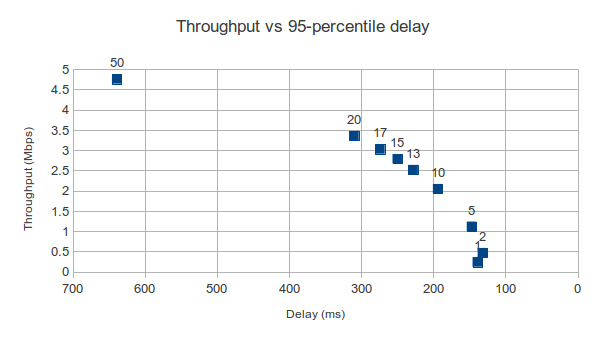
\includegraphics[width=1\textwidth]{fixedWindow.png}
  \end{center}
 \caption{Throughput vs 95-percentile delay with a fixed window size}
 \label{fig:fixedWindow}
\end{figure}

Our first try to implement an AIMD scheme did not produce very good results; we got
-5.84 log(Throughput/Delay) when adding $ 1/w $ to the window size on
every ACK and dividing by 2 on every timeout (timeout set to 1000 ms). A slower 
increase of $ 1/w^2 $ improved the score to -4.72. Another approach we tried was to
change the timeout, where we found out that decreasing the timeout to 100 ms improves
the score to -5.28 (while maintaining the standard AIMD). By combining both approaches
we managed to improve the score up to -4.12, by using a timeout of 100 ms, an additive 
increase of $ 1/w^2 $ on every ACK, and a harsher decrease of $ w \leftarrow \sqrt{w} $ 
on every timeout.

The delay-triggered scheme proved to be competitive with AIMD. We experimented with 
changing the window size based on when the RTT crosses a given threshold. 
Table~\ref{tab:delayTriggered} summarizes the results. The best score of -4.16 was achieved with a threshold 
of 100 ms, an increase of 0.1,\footnote{A non-integer increase effectively means 
that the window size changes only when it reaches the following integer} and a 
decrease of 1.

\begin{table}[h]
 \centering
 \begin{tabular}{|l|l|l|l|p{2cm}|l|}
 \hline
   Threshold (ms) & Increase & Decrease & Delay (ms) & Throughput (Mbps) & Score \\
 \hline
  100 & 1 & 1 & 308 & 3.39 & -4.51 \\
  200 & 1 & 1 & 580 & 4.02 & -4.97 \\
  50  & 1 & 1 & 162 & 1.75 & -4.53 \\
  100 & 2 & 2 & 436 & 3.76 & -4.75 \\
  100 & 1 & 2 & 299 & 3.12 & -4.56 \\
  100 & 0.1 & 1 & 155 & 2.41 & -4.16 \\
  \hline
 \end{tabular}
 \caption{Delay, throughput, and log(Throughput/Delay) score with different 
 delay-triggered schemes.}
 \label{tab:delayTriggered}
\end{table}

\section{Contest}
One approach we tried was to change the window size based on changes in the delivery time, 
i.e. the one-way trip time from the sender to the receiver. The assumption was that since we 
are only messured on this direction, we shouldn't include delays in receiving ACKs in 
the calculation. A first attempt was to compare the delivery time of the current acked
packet to that of the previous packet. If the difference in delivery times was significant, 
we adapt the window size. Specifically, if the current delivery time is less than half
of the previous delivery time, we increase the window size by one. If the current 
delivery time is more than two times the previous time, we decrease it by one; otherwise 
we do nothing. This scheme achieved a score of -4.53 (165 ms delay, 1.77 Mbps throughput). 

Next we tried to reduce the frequency of changes, such that we compare to a previous 
delivery time only after a certain period of time has passed. Doing this every 100 ms 
reduced the delay (to 141 ms) but also drastically hurt the throughout (0.54 Mbps), 
and achieved a score of -5.74. We therefore decided to increase the window size more 
often, and combined our approach with an AIMD scheme, such that we increase the window 
size on every ACK, decrease on every timeout,
\footnote{The timeout was set to 100 ms based on the results from the previous section. 
A sanity check showed that a 1000 ms timeout produces much worse results.} 
but also adapt it based on comparing the current delivery time with a previous one. 
We managed to achieve a score of -4.14 (167 ms delay, 2.65 Mbps throughput) with the 
following parameters: 

\begin{enumerate}
 \item On every ACK, $ w \leftarrow w + 1/w^2 $.
 \item On every timeout, $ w \leftarrow \sqrt[4]{w} $.
 \item Every 200 ms, compare the current delivery time to a 200-ms-ago delivery time. 
 $ \textsf{If cur} < 0.5 * \textsf{prev}, w \leftarrow w-1$. $ \textsf{If cur} > 2 * 
 \textsf{prev}, w \leftarrow w+1 $. 
\end{enumerate}

Another attempt we made was based on the assumption that delivery times of individual 
packets may fluctuate, and we don't want to make changes based on inconsistent 
fluctuations. We therefore messured the average delivery time of the last $k$ packets,
and compared it with the average delivery time of the $k$ packets that preceded them. 
The change in the window size was then made in a similar manner: if the current average
delivery time was larger than the previous, we increment the window size; otherwise we 
decrement it. With this scheme we achieved a very low delay (107 ms) but at the cost
of a low throughput (1.16 Mbps), with a combined score of -4.52. 


\end{document}